\documentclass{cours}
\usepackage{tkz-tab}

\title{Fonctions Trigonométriques}

\begin{document}
    \maketitle{17}

    \begin{Gpartie}{Définition et Propriétés} 
        \begin{Spartie}{Rappel} 
            Soit un réel $x$ et $M$ le point correspondant sur le cercle trigonométrique dans une repère orthonormé $\left(~O~;~\vec{\imath}~,~\vec{\jmath}~\right)$

            Le cosinus de $x$ est noté $\cos(x)$, où $\cos(x)$ est l'abscisse du point $M$. \\
            Le sinus de $x$ est noté $\sin(x)$, où $\sin(x)$ est l'ordonnée du point $M$.
            
            \begin{center}
                % \begin{tikzpicture}
                    \includegraphics[width=10cm]{example-image}
                % \end{tikzpicture}
                \parbox{\linewidth}{\captionof{figure}{\centering Cercle Trigonométrique}}
            \end{center}
        \end{Spartie}
        \begin{Spartie}{Définitions} 
            La fonction qui à tout réel $x$ associe le nombre $\cos(x)$ est appelée fonction cosinus. \\
            La fonction qui à tout réel $x$ associe le nombre $\sin(x)$ est appelée fonction sinus.
        \end{Spartie}
        \begin{Spartie}{Propriété} 
            Quel que soit le réel $x$, $\cos(-x)=\cos(x)$, la fonction est donc paire. \\
            Quel que soit le réel $x$, $\sin(-x)=-\sin(x)$, la fonction est donc impaire.
        \end{Spartie}
        \begin{Spartie}{Propriété (Periodicité)} 
            Pour tout réel $x$, $\cos(x+2\pi)=\cos(x)$ et $\sin(x+2\pi)=\sin(x)$

            Les fonctions cosinus et sinus sont donc périodiques de période $2\pi$ ($2\pi$-périodiques)
        \end{Spartie}
        \begin{Spartie}{Remarque} 
            Ces deux propriétés permettent de réduire l'intervalle d'étude des fonctions cosinus et sinus à $\big[~0~;~\pi~\big]$

            Par parité, on peut déduire $\big[~-\pi~;~0~\big]$, donc $\big[~-\pi~;~\pi~\big]$.
            
            Par périodicité on peut déduire les résultats sur $\mathbb{R}$
        \end{Spartie}
    \end{Gpartie}
    \begin{Gpartie}{Dérivabilité} 
        \begin{Spartie}{Étude des Fonctions Sinus et Cosinus} 
            \begin{SSpartie}{Théorème} 
                Les fonctions sinus et cosinus sont dérivables sur $\mathbb{R}$, et pour tout réel $x$ : \[\sin'(x)=\cos(x)\quad\text{et}\quad\cos'(x)=-\sin(x)\]
            \end{SSpartie}
            \begin{SSpartie}{Tableaux de Variation} 
                \begin{center}
                    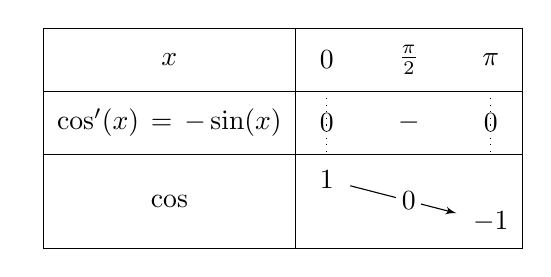
\begin{tikzpicture}[scale=0.8]
                        \tkzTabInit[lgt=4, espcl=1.3]{$x$ /1 , $\cos'(x)=-\sin(x)$ /1 , $\cos$ /1.5}{$0$ , $\frac{\pi}{2}$ , $\pi$}
                        \tkzTabLine{ z ,  , - ,  , z }
                        \tkzTabVar{ + / $1$ , R , - / $-1$}
                        \tkzTabVal{1}{3}{0.5}{}{0}
                    \end{tikzpicture}
                    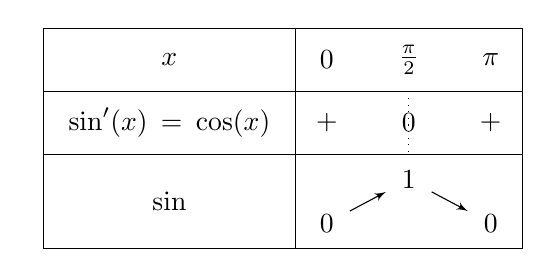
\begin{tikzpicture}[scale=0.8]
                        \tkzTabInit[lgt=4, espcl=1.3]{$x$ /1 , $\sin'(x)=\cos(x)$ /1 , $\sin$ /1.5}{$0$ , $\frac{\pi}{2}$ , $\pi$}
                        \tkzTabLine{ + ,  , z ,  , + }
                        \tkzTabVar{ - / $0$ , + / $1$ , - / $0$}
                    \end{tikzpicture}
                    \parbox{\linewidth}{\captionof{figure}{\centering Tableaux de Variation des Fonctions cosinus et sinus}}
                \end{center}
            \end{SSpartie}
            \begin{SSpartie}{Courbes Représentatives} 
                \begin{center}
                    % \begin{tikzpicture}
                        \includegraphics[width=10cm]{example-image}
                    % \end{tikzpicture}
                    \parbox{\linewidth}{\captionof{figure}{\centering Représentation Graphique des Fonctions cosinus et sinus}}
                \end{center}
            \end{SSpartie}
        \end{Spartie}
        \begin{Spartie}{Complément} 
            \begin{SSpartie}{Théorème} 
                \[\lim\limits_{x\to0}\frac{\sin(x)}{x}=1\] \[\lim\limits_{x\to0}\frac{\cos\left(x-\frac{\pi}{2}\right)}{x}=1\]
                \begin{SSSpartie}{Démonstration} 
                    La fonction sinus est continue et dérivable en $0$ : \[\lim\limits_{h\to0}\frac{\sin(0+h)-\sin(0)}{h}=\sin'(0)=\cos(0)=1\] \[\lim\limits_{h\to0}\frac{\cos\left(-\frac{\pi}{2}+h\right)-\cos\left(-\frac{\pi}{2}\right)}{h}=\cos'\left(-\frac{\pi}{2}\right)=-\sin\left(-\frac{\pi}{2}\right)=1\]
                \end{SSSpartie}
            \end{SSpartie}
        \end{Spartie}
    \end{Gpartie}
\end{document}